
%================================
\subsection{Resultados de la implementación con MPI con optimizaciones por compilador}
\label{sec:Resultados de la implementación con MPI con optimizaciones por compilador}

Estos son los resultados obtenidos con la implementación con MPI con optimización por compilador usando las flags mencionadas en la sección ~\ref{pruebas} ejecutado en las maquinas de AWS antes mencionadas.


\begin{table}[H]
   \centering
   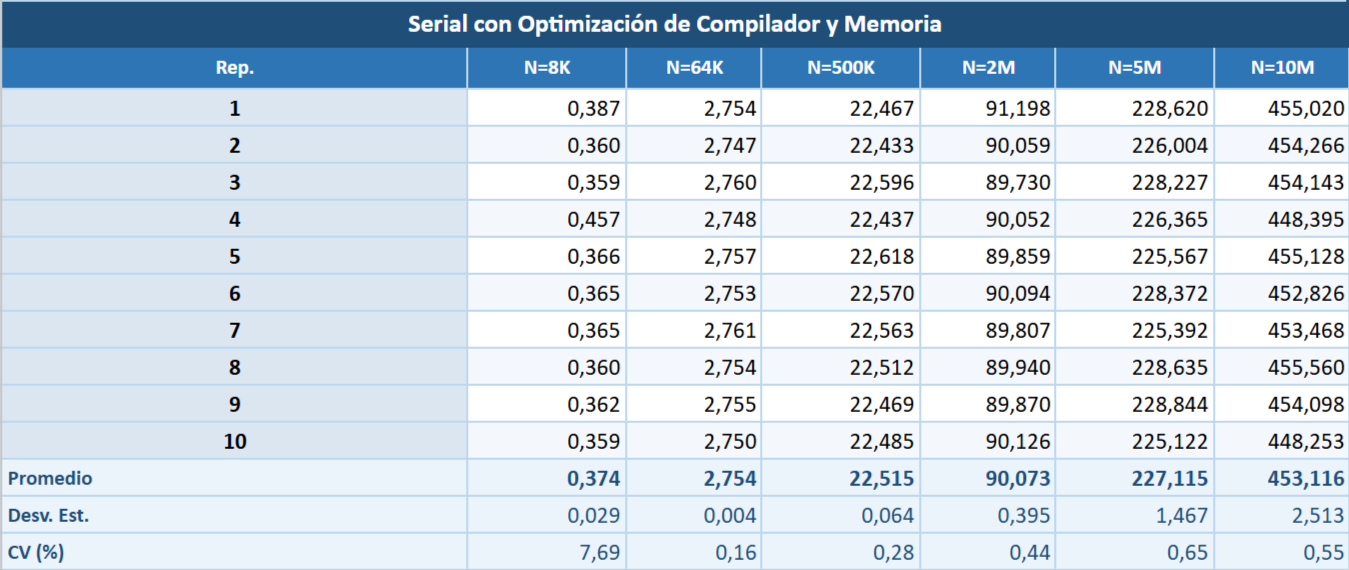
\includegraphics[width=1\textwidth]{images/tables/time_mpi_2_opt.png}
   \caption{Tiempos de ejecución de la implementación con MPI con 2 procesos}
\end{table}

\begin{table}[H]
   \centering
   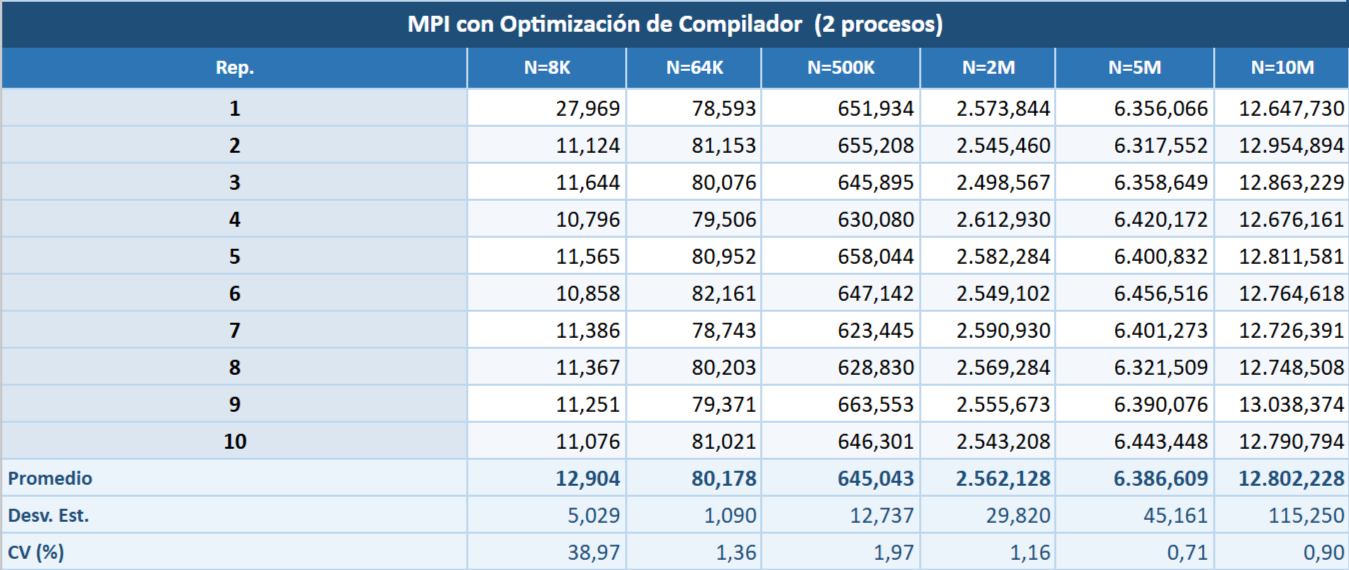
\includegraphics[width=1\textwidth]{images/tables/time_mpi_3_opt.png}
   \caption{Tiempos de ejecución de la implementación con MPI con 3 procesos}
\end{table}

\begin{table}[H]
   \centering
   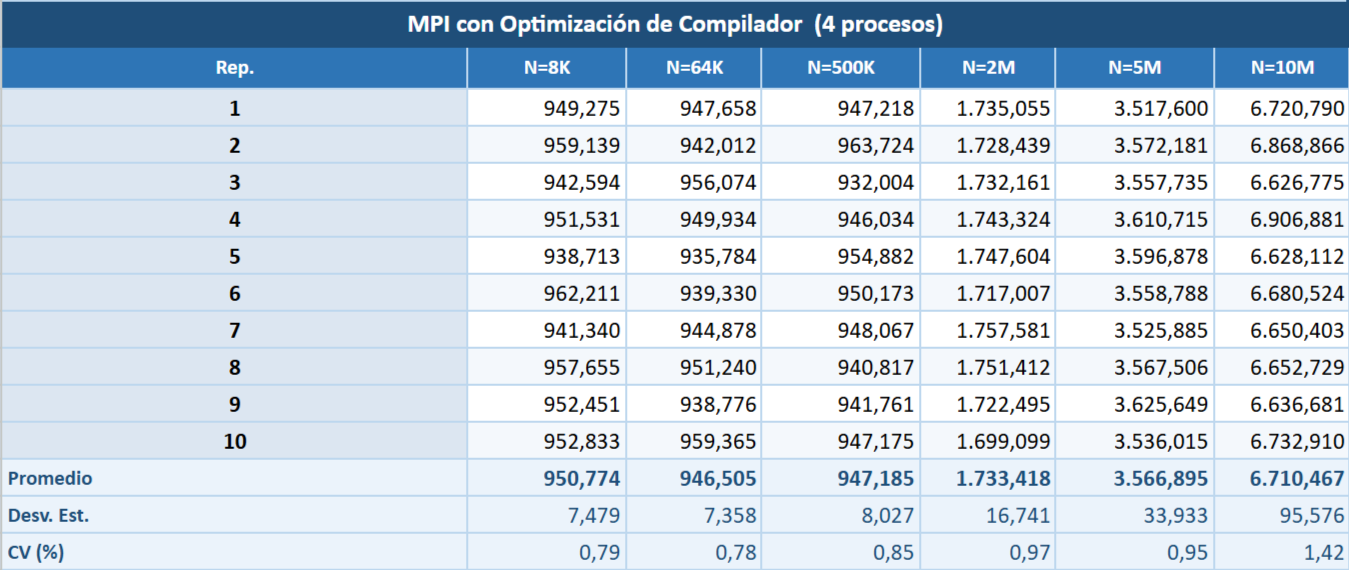
\includegraphics[width=1\textwidth]{images/tables/time_mpi_4_opt.png}
   \caption{Tiempos de ejecución de la implementación con MPI con 4 procesos}
\end{table}

\begin{table}[H]
   \centering
   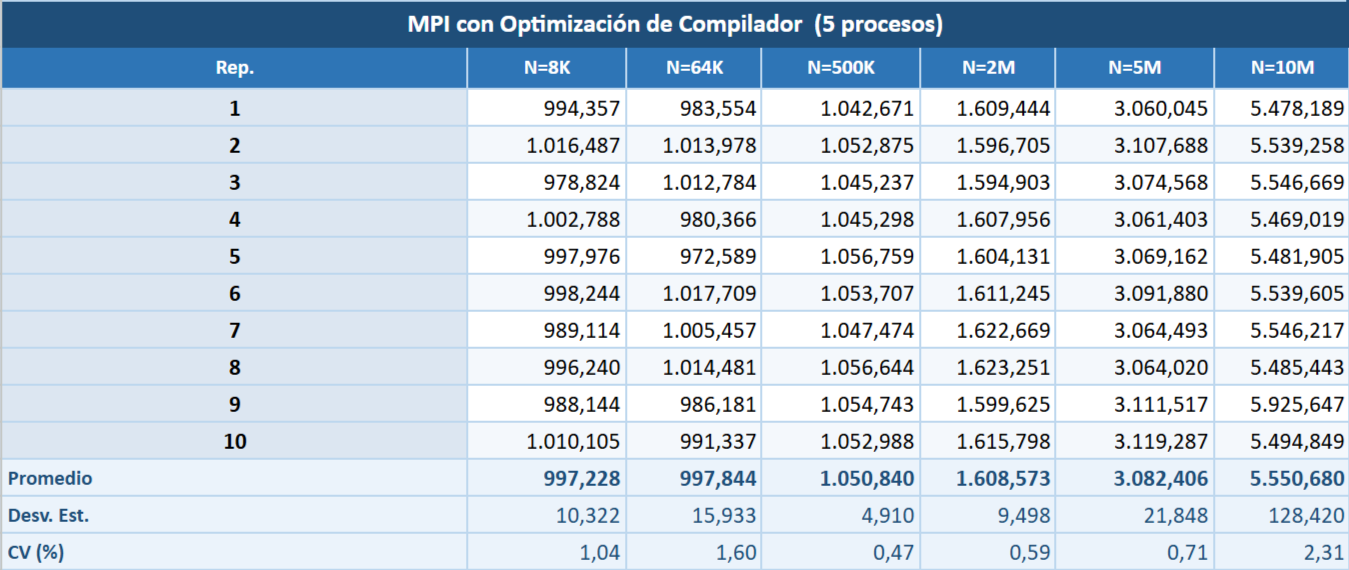
\includegraphics[width=1\textwidth]{images/tables/time_mpi_5_opt.png}
   \caption{Tiempos de ejecución de la implementación con MPI con 5 procesos}
\end{table}

\begin{table}[H]
   \centering
   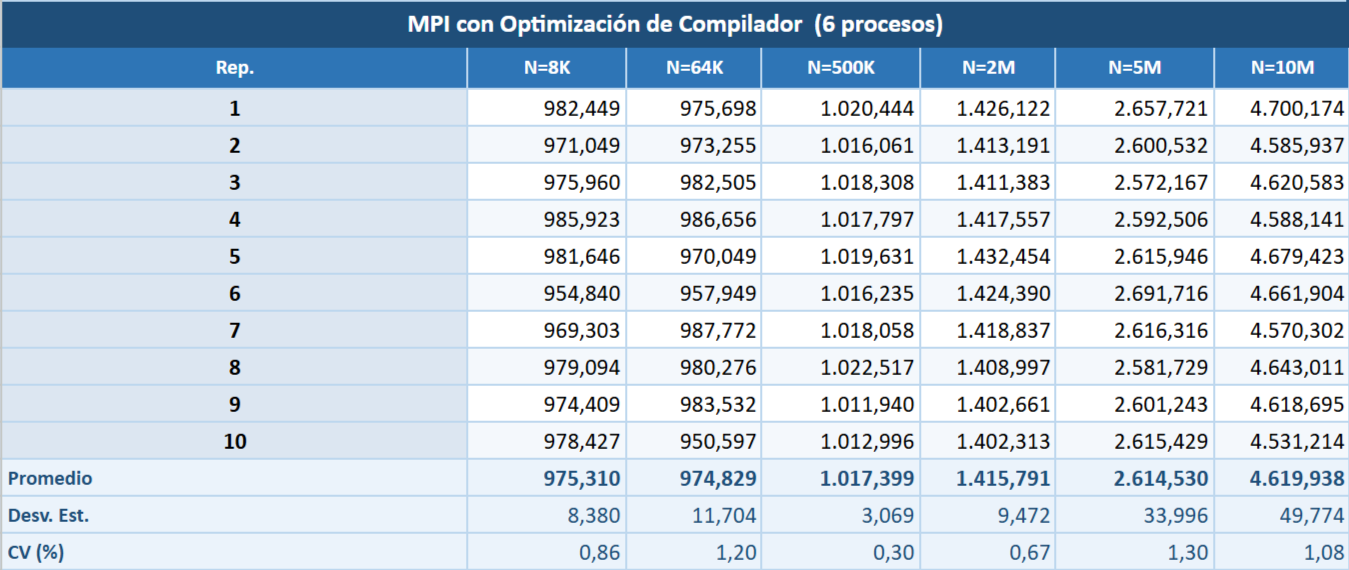
\includegraphics[width=1\textwidth]{images/tables/time_mpi_6_opt.png}
   \caption{Tiempos de ejecución de la implementación con MPI con 6 procesos}
\end{table}

\begin{figure}[H]
   \centering
   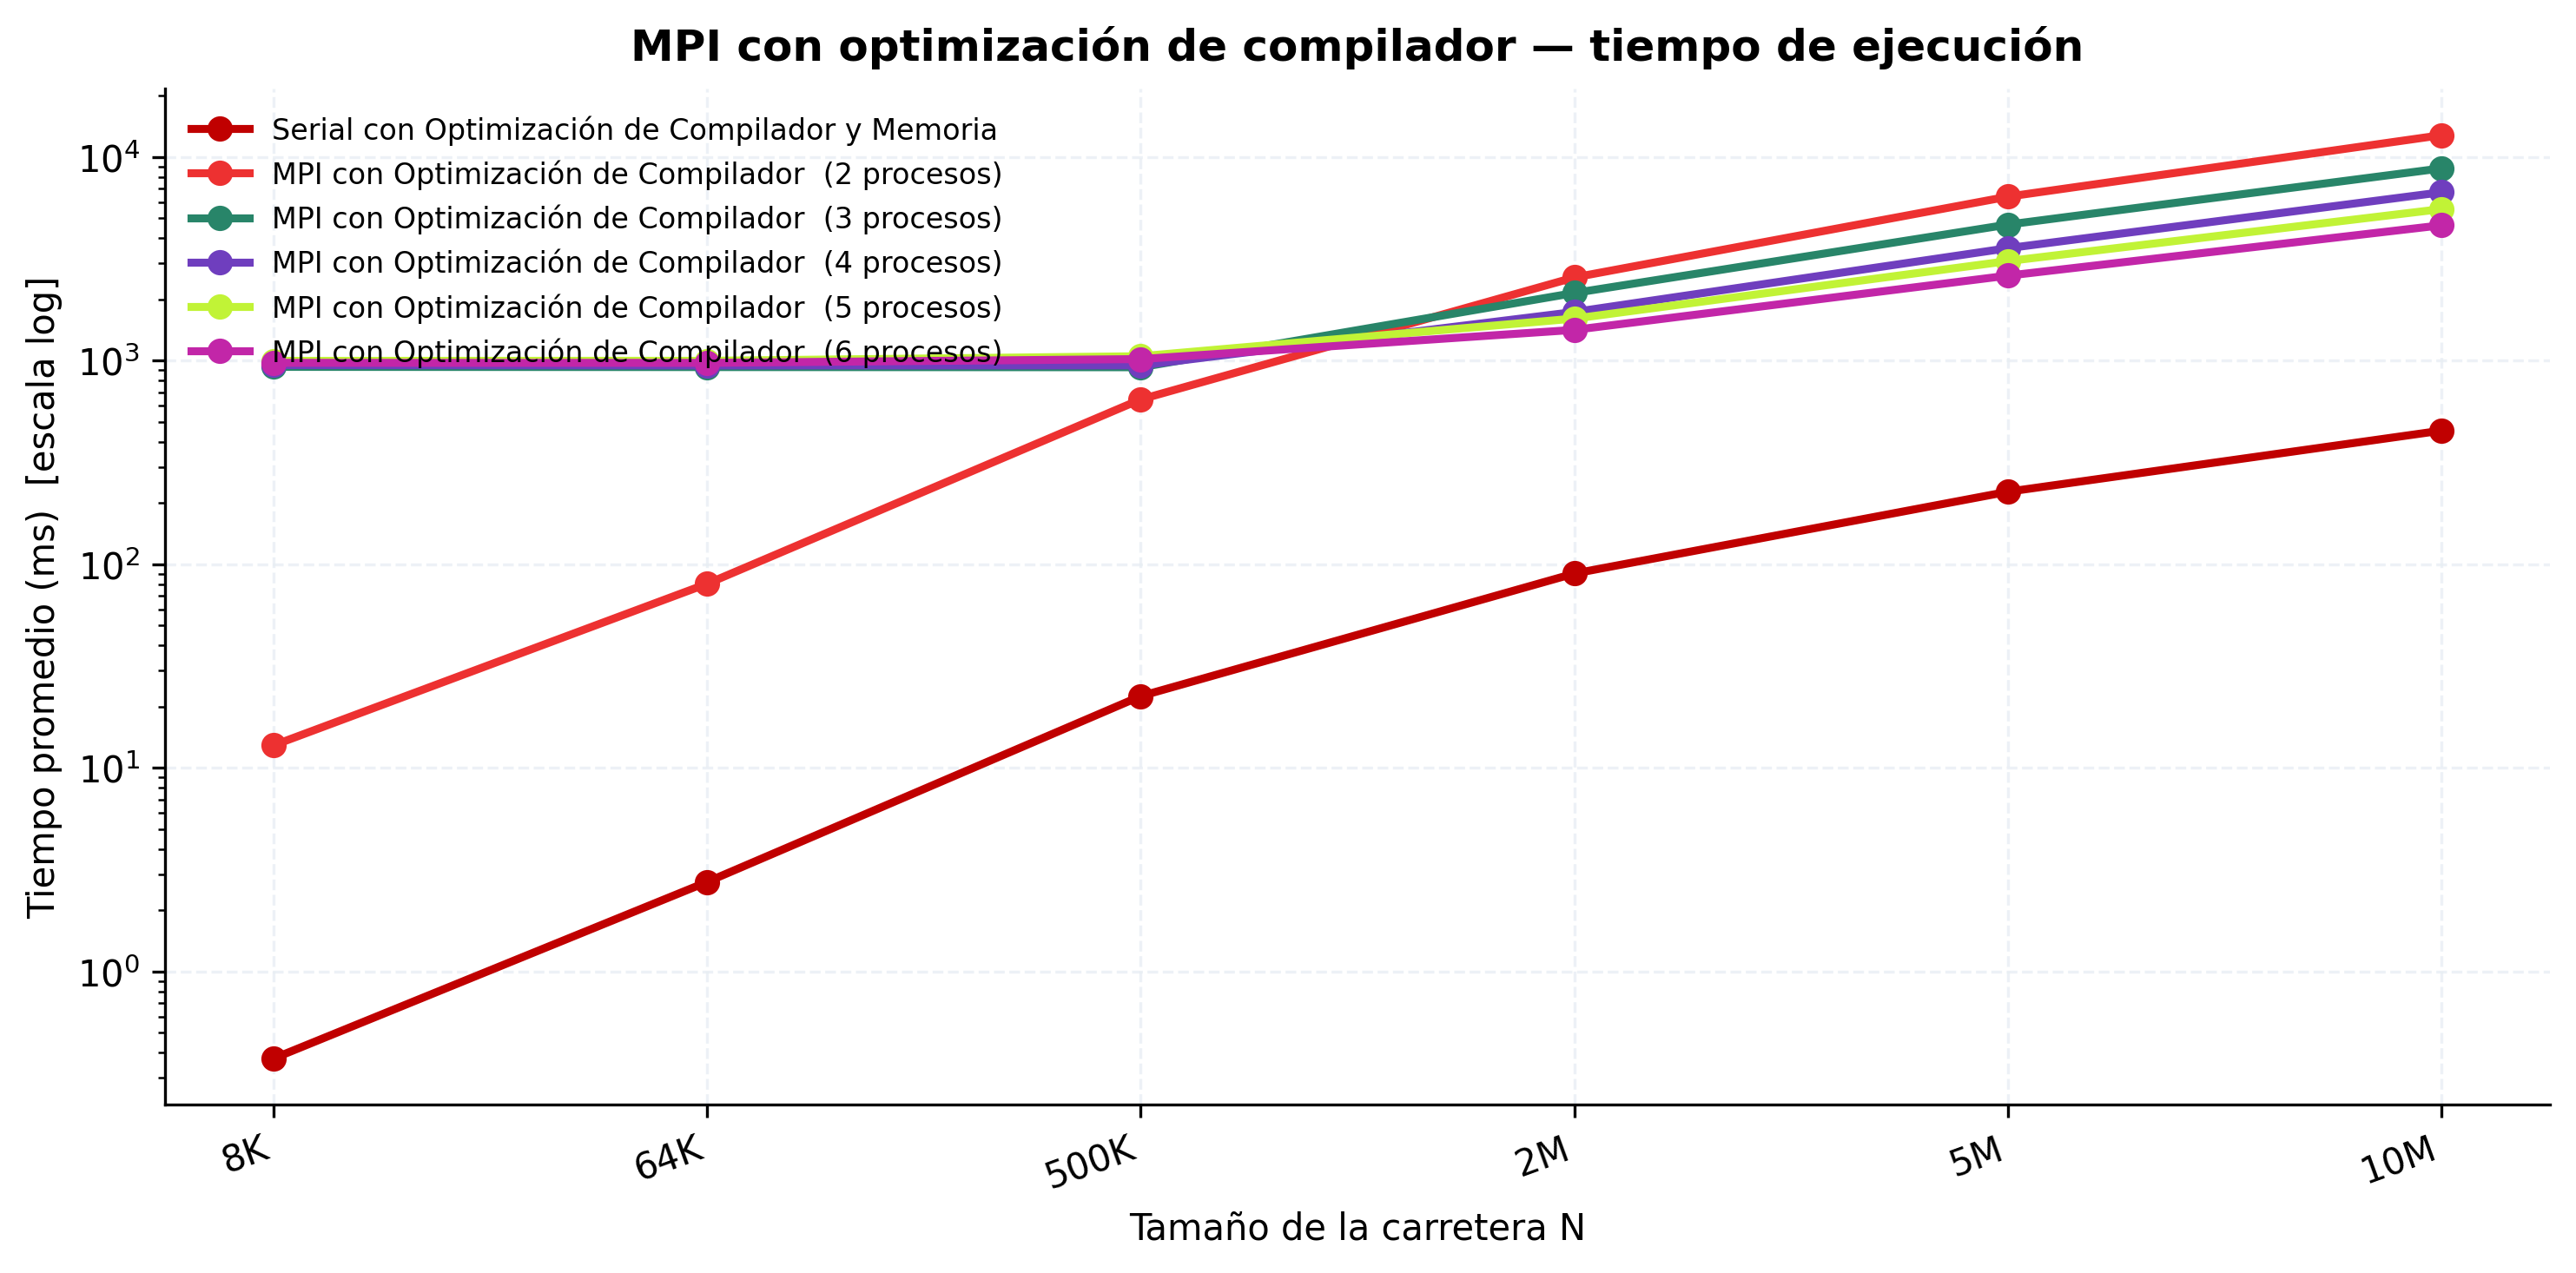
\includegraphics[width=1\textwidth]{images/charts/time_mpi_opt.png}
   \caption{Gráfica de tiempos de la implementación con MPI con optimización}
\end{figure}

\begin{table}[H]
   \centering
   
\includegraphics[width=1\textwidth]{images/tables/speedup_mpi_opt.png}
   \caption{Speedup de la implementación con MPI con optimización}
\end{table}

\begin{figure}[H]
   \centering
   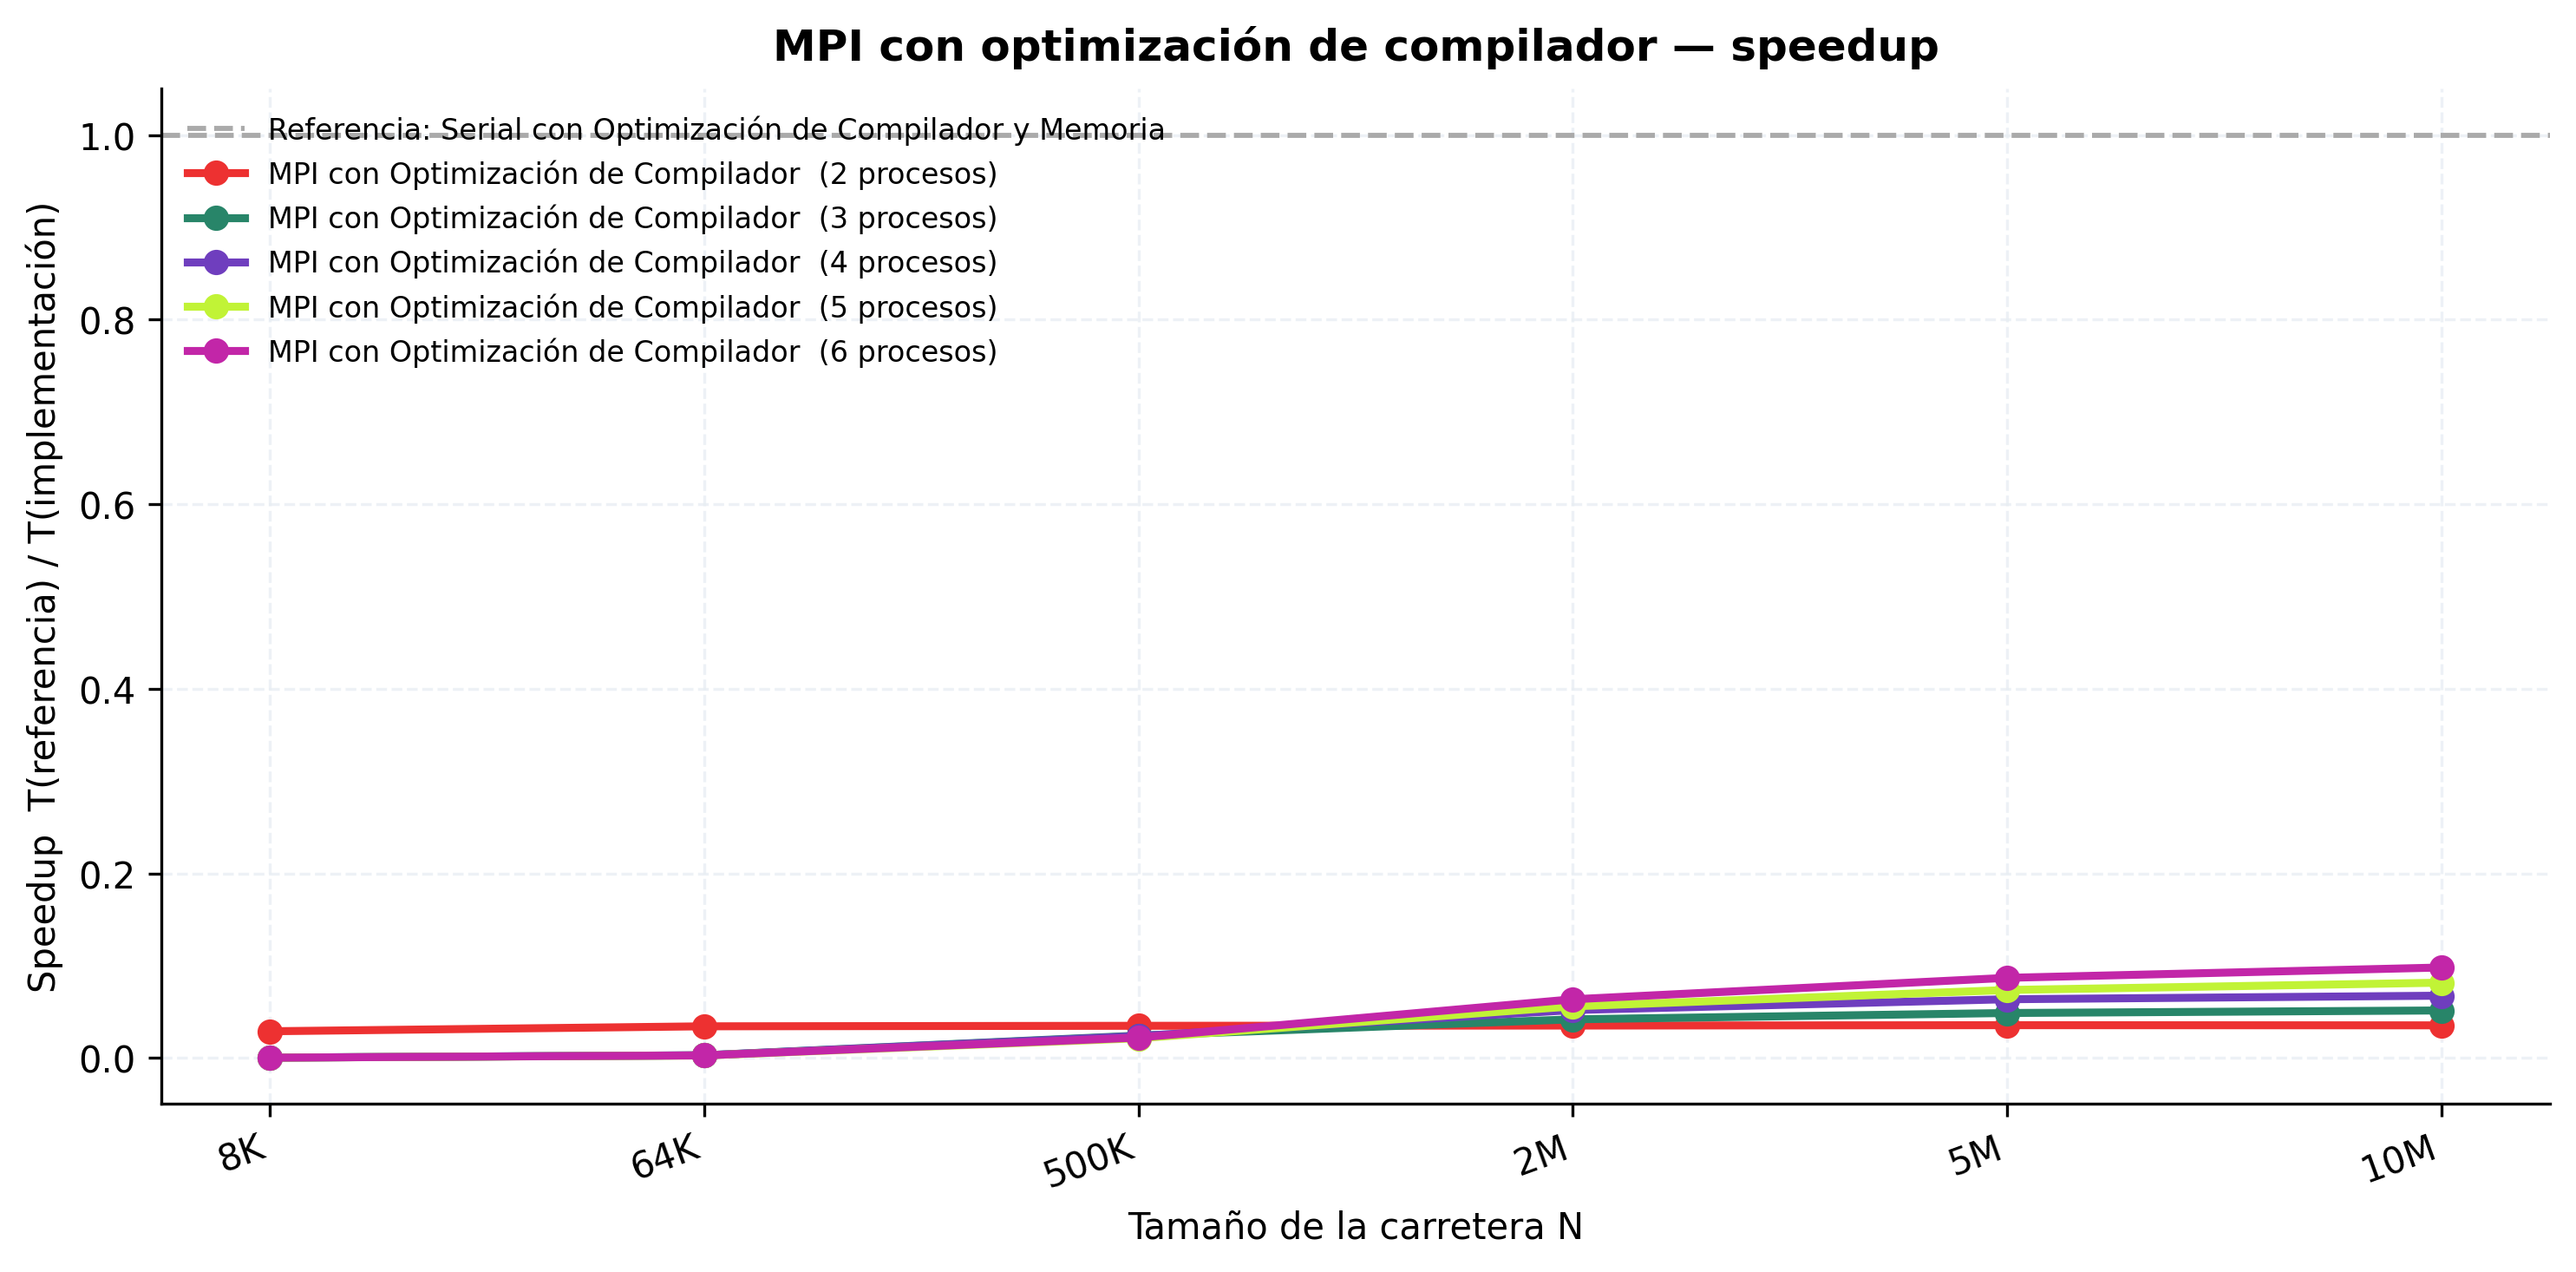
\includegraphics[width=1\textwidth]{images/charts/speedup_mpi_opt.png}
   \caption{Gráfica de Speedup de la implementación con MPI con optimización}
\end{figure}
